
%(BEGIN_QUESTION)
% Copyright 2006, Tony R. Kuphaldt, released under the Creative Commons Attribution License (v 1.0)
% This means you may do almost anything with this work of mine, so long as you give me proper credit

Bestem en enkel 5-punkts (0\%, 25\%, 50\%, 75\% og 100\%) kalibreringstabell for fortrenger-nivåtransmitteren i dette scenariet:

$$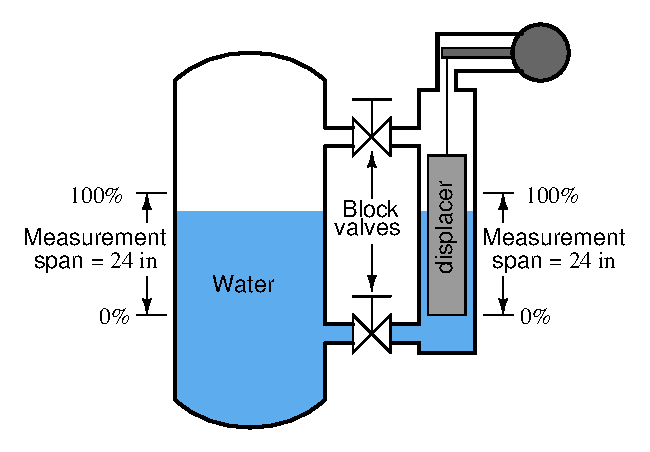
\includegraphics[width=15.5cm]{i00278x01.eps}$$

Den sylindriske fortrengeren veier 10 pund (tørr) og har diameter 3 tommer.  Prosessvæsken er vann (tetthet = 62.428 lb/ft$^{3}$).  0\% prosessnivå (LRV) er ved bunnen av fortrengeren.  Anta pneumatisk transmittermekanisme med utgangsområde 3 til 15 PSI, og kalibreringstoleranse +/- 1\% (av spenn).

% No blank lines allowed between lines of an \halign structure!
% I use comments (%) instead, so that TeX doesn't choke.

$$\vbox{\offinterlineskip
\halign{\strut
\vrule \quad\hfil # \ \hfil & 
\vrule \quad\hfil # \ \hfil & 
\vrule \quad\hfil # \ \hfil & 
\vrule \quad\hfil # \ \hfil & 
\vrule \quad\hfil # \ \hfil & 
\vrule \quad\hfil # \ \hfil \vrule \cr
\noalign{\hrule}
%
% First row
Prosess- & Prosent av & Oppdrifts- & Utgangssignal & Utgangssignal & Utgangssignal \cr
%
% Another row
nivå (in) & spenn (\%) & kraft (lb) & ideelt (PSI) & min. (PSI) & maks. (PSI) \cr
%
\noalign{\hrule}
%
% Another row
  & 0 &  &  &  &  \cr
%
\noalign{\hrule}
%
% Another row
  & 25 &  &  &  &  \cr
%
\noalign{\hrule}
%
% Another row
  & 50 &  &  &  &  \cr
%
\noalign{\hrule}
%
% Another row
  & 75 &  &  &  &  \cr
%
\noalign{\hrule}
%
% Another row
  & 100 &  &  &  &  \cr
%
\noalign{\hrule}
} % End of \halign 
}$$ % End of \vbox

\underbar{file i00278}
%(END_QUESTION)





%(BEGIN_ANSWER)

% No blank lines allowed between lines of an \halign structure!
% I use comments (%) instead, so that TeX doesn't choke.

$$\vbox{\offinterlineskip
\halign{\strut
\vrule \quad\hfil # \ \hfil & 
\vrule \quad\hfil # \ \hfil & 
\vrule \quad\hfil # \ \hfil & 
\vrule \quad\hfil # \ \hfil & 
\vrule \quad\hfil # \ \hfil & 
\vrule \quad\hfil # \ \hfil \vrule \cr
\noalign{\hrule}
%
% First row
Prosess- & Prosent av & Oppdrifts- & Utgangssignal & Utgangssignal & Utgangssignal \cr
%
% Another row
nivå (in) & spenn (\%) & kraft (lb) & ideelt (PSI) & min. (PSI) & maks. (PSI) \cr
%
\noalign{\hrule}
%
% Another row
0  & 0 & 0 & 3 & 2.88 & 3.12 \cr
%
\noalign{\hrule}
%
% Another row
6 & 25 & 1.532 & 6 & 5.88 & 6.12 \cr
%
\noalign{\hrule}
%
% Another row
12 & 50 & 3.064 & 9 & 8.88 & 9.12 \cr
%
\noalign{\hrule}
%
% Another row
18 & 75 & 4.597 & 12 & 11.88 & 12.12 \cr
%
\noalign{\hrule}
%
% Another row
24 & 100 & 6.129 & 15 & 14.88 & 15.12 \cr
%
\noalign{\hrule}
} % End of \halign 
}$$ % End of \vbox


%(END_ANSWER)





%(BEGIN_NOTES)


%INDEX% Calibration: table, level transmitter
%INDEX% Measurement, level: calibration table
%INDEX% Measurement, level: displacer (buoyancy)

%(END_NOTES)
